\documentclass{article}

% For visualization.
\usepackage{graphicx} 

% For citations
\usepackage[authoryear,round]{natbib}

% For algorithms
\usepackage{amsmath}
\usepackage{amsthm}
\usepackage{authblk}

\hyphenation{general-iza-tions}
\hyphenation{distri-bution}
\hyphenation{Zel-ter-man}

\newtheorem{lemma}{Lemma}
\newtheorem{corollary}{Corollary}
\newtheorem{prop}{Proposition}
\newtheorem{thm}{Theorem}

\begin{document}

\title{SNB Results Paper 2}

\author{Michael J. Kane}
\author{Daniel Zelterman}

\affil{Department of Biostatistics, Yale University, New Haven CT, USA}

\maketitle

%\begin{abstract}
%This paper other properties of the snb...
%\end{abstract}

\section{The Stopped Negative Binomial Distribution} \label{sect:intro}

\begin{enumerate}
\item Review of the SNB
\item Show when the SNB is and isn't unimodel.
\item Past efforts to show the asymptotic behavior using Sterling 
approximations.
\end{enumerate}

\section{Main Proof}

\begin{thm} \label{thm:main}
The main theorem states that once there is a central limit effect 
then the hitting times look the L\'{e}vy-Bachlier formula for the density 
of the first hitting time of a sloped line.
\end{thm}

The proof of Theorem \ref{thm:main} proceeds as follows. In Section
\ref{sect:process_construction} it is shown that the SNB can be 
constructed as a binomial process on a grid. Under suitable 
rotation and scaling the process is equivalent to a random walk 
on the integers with stopping rules. Section \ref{sect:fclt} shows that
after reparameterizing the process it converges to a Standard Brownian
Motion with stopping rules. The density of the first hitting times for
the two separate endpoints are each distributed according to the 
L\'{e}vy-Bachlier formula. Section \ref{sect:stat} provides statistical 
results, deriving the convergence when the rotation and scaling parameters
are estimated from data. Section \ref{sect:discussion} ends the article
with a discussion and proposes avenues for future work.

\section{Process Construction} \label{sect:process_construction}

As shown in Section \ref{sect:intro} the SNB can be conceptualized as
a series of coin flips that stop when either $s$ heads or $t$ tail are
reached. The time to reach either $s$ or $t$ is distributed as the SNB.
The process can be visualized as in Figure \ref{z-plot1.pdf}. The process
starts at the origin and at each step a coin is flipped if it is heads
the process moves in the vertical direction one step, if tails it moves
one step in the horizontal direction.

\begin{figure}[ht]
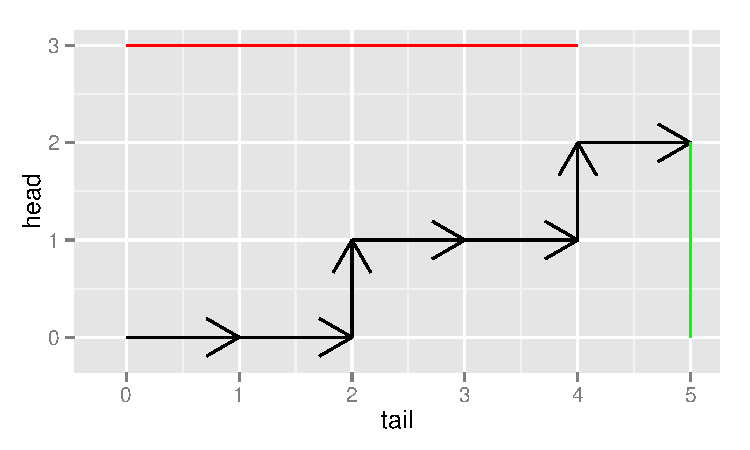
\includegraphics[width=\textwidth]{z-plot1.pdf}
\caption{
A hypothetical realization of the SNB coin-flipping process.
}
\label{fig:z_plot}
\end{figure}

The expected slope of the process is determined by $p \in [0, 1]$, the 
probability of a heads. If $s$ and $t$ are finite, then as $p$ increases 
the probability a given realization of the process hits $s$ increases (and
$t$ decreases). Likewise as the $p$ decreases the probability a realization 
hits $s$ decreases (and $t$ increases).

Letting $p = \alpha / \alpha + \beta$, the expected direction of the 
process is $\theta = \text{atan}(\alpha / \beta)$. In Section \ref{sect:stat}
it is shown that an estimate of $\theta$ converges at the same rate as
an estimate of $p$. For now though, we would like to rotate the process
clockwise by $\theta$ so that, in expectation, the rotate process angle
is zero.

\begin{lemma}
After rotation, the line $y=s$ becomes
\begin{equation}
y' = -\tan(\theta) x' + s \left(\sin(\theta) \tan(\theta) + \cos(\theta) \right)
\end{equation}
where $y'$ and $x'$ are the vertical and horizontal axes in the rotation
space.
\end{lemma}

\begin{enumerate}
\item Show a picture of the z-plot before and after rotation/rescaling.
\item Rotate the system clockwise by $\theta = p = \alpha/(\alpha+\beta)$ 
where $\beta$ is the number of failures and $\alpha$ is the number of successes.
\item Derive the rotated $t$- and $s$-lines.
\item Calculate the scaling for the rotated $t$- and $s$- lines so that the
reparameterized process goes right and either up on step or down one step...
Like a random walk on the integers over time.
\end{enumerate}

\section{The FCLT for the process} \label{sect:fclt}

\begin{enumerate}
\item TODO: Find the appropriate scalings for $s$ an $t$ in terms of $n$
\item Use the Heyde/Hall FCLT to show that the symmetric random walk
converges to a Standard Brownian motion over the appropriate interval.
\item Derive the probability of hitting $s$ or $t$ as a Girsinov process.
\end{enumerate}

Describe the properties of the Girsinov process and relate them back to 
the multi-mode result from the beginning.

\section{Estimating $\theta$ and the rotations from data} \label{sect:stat}

\begin{enumerate}
\item Show that if we need to estimate $\theta$ that it converges like 
$\widehat{p}$. Include the graph of $\widehat{\theta}$ vs. $\alpha$.
\item Show convergence results for for the $s$- and $t$-lines. 
\end{enumerate}

\section{Discussion and Future Work} \label{sect:discussion}

\bibliography{references}
\bibliographystyle{jss}

\end{document}
